\documentclass[aspectratio=169,12pt]{beamer}

% Theme and colors
\usetheme{Madrid}
\usecolortheme{whale}
\setbeamertemplate{navigation symbols}{}
\setbeamertemplate{footline}[frame number]

% Packages
\usepackage{amsmath,amssymb}
\usepackage{graphicx}
\usepackage{tikz}
\usetikzlibrary{shapes,arrows.meta,positioning,calc,decorations.pathreplacing}
\usepackage{booktabs}
\usepackage{array}
\usepackage{xcolor}
\usepackage{hyperref}

% Custom colors
\definecolor{codegreen}{rgb}{0,0.6,0}
\definecolor{codepurple}{rgb}{0.58,0,0.82}
\definecolor{darkblue}{rgb}{0,0,0.7}

\title[Video Compression \& MPEG]{Video Compression and MPEG Standards}
\subtitle{Motion Compensation, MPEG-1, 2, 4, and 7}
\author[Mahesh C]{\textbf{Mahesh C}\\FISAT}
\institute{Federal Institute of Science and Technology (FISAT)\\Multimedia Technology Class}
\date{\today}

\begin{document}

\begin{frame}
    \titlepage
    \begin{center}
        \small Based on: Li \& Drew, \textit{Fundamentals of Multimedia}, Pearson Education, 2004
    \end{center}
\end{frame}

\begin{frame}{Outline}
    \tableofcontents
\end{frame}


%==============================================================================
\section{Video Compression Based on Motion Compensation}
%==============================================================================

\begin{frame}{Why Video Compression?}
    \textbf{Raw video is enormous:}
    \begin{itemize}
        \item 1 frame at 720$\times$480, 24-bit color = 1.04 MB
        \item At 30 fps $\rightarrow$ 31.1 MB/s $\rightarrow$ 1.87 GB/min
        \item A 2-hour movie $\rightarrow$ \textbf{224 GB} uncompressed!
    \end{itemize}
    
    \vspace{0.3cm}
    \begin{block}{Key Observation}
        Consecutive video frames are very similar. Most of the scene stays the same from frame to frame.
    \end{block}
    
    \vspace{0.3cm}
    \textbf{Two types of redundancy:}
    \begin{itemize}
        \item \textbf{Spatial redundancy:} Within a single frame (like JPEG)
        \item \textbf{Temporal redundancy:} Between consecutive frames
    \end{itemize}
\end{frame}

\begin{frame}{Temporal Redundancy}
    \begin{center}
        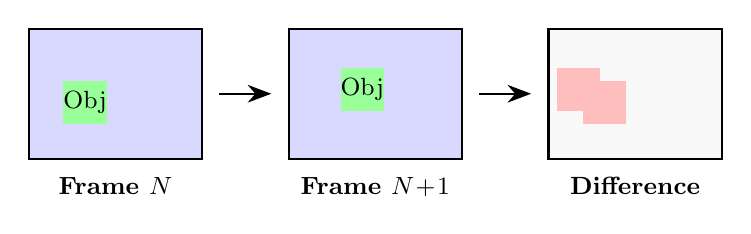
\begin{tikzpicture}[scale=0.55]
            % Frame N
            \fill[blue!15] (0,0) rectangle (4,3);
            \fill[green!40] (0.8,0.8) rectangle (1.8,1.8);
            \draw[thick] (0,0) rectangle (4,3);
            \node[font=\small] at (1.3,1.3) {Obj};
            \node[below,font=\small\bfseries] at (2,-0.2) {Frame $N$};
            
            % Arrow
            \draw[-{Stealth[length=3mm]},thick] (4.4,1.5) -- (5.6,1.5);
            
            % Frame N+1
            \fill[blue!15] (6,0) rectangle (10,3);
            \fill[green!40] (7.2,1.1) rectangle (8.2,2.1);
            \draw[thick] (6,0) rectangle (10,3);
            \node[font=\small] at (7.7,1.6) {Obj};
            \node[below,font=\small\bfseries] at (8,-0.2) {Frame $N\!+\!1$};
            
            % Arrow
            \draw[-{Stealth[length=3mm]},thick] (10.4,1.5) -- (11.6,1.5);
            
            % Difference
            \fill[gray!5] (12,0) rectangle (16,3);
            \fill[red!25] (0.8+12,0.8) rectangle (1.8+12,1.8);
            \fill[red!25] (7.2+5,1.1) rectangle (8.2+5,2.1);
            \draw[thick] (12,0) rectangle (16,3);
            \node[below,font=\small\bfseries] at (14,-0.2) {Difference};
        \end{tikzpicture}
    \end{center}
    
    \vspace{0.3cm}
    \textbf{Most of the difference frame is zero} (empty).
    
    Only the moving object creates non-zero values.
    
    \vspace{0.2cm}
    \textit{If we predict the next frame, we only need to store the small difference!}
\end{frame}

\begin{frame}{Motion Compensation: The Core Idea}
    \begin{block}{Principle}
        Instead of storing each frame independently, store:
        \begin{enumerate}
            \item A \textbf{reference frame} (full image)
            \item \textbf{Motion vectors} (MV) describing how blocks moved
            \item A small \textbf{residual} (prediction error)
        \end{enumerate}
    \end{block}
    
    \vspace{0.3cm}
    \begin{center}
        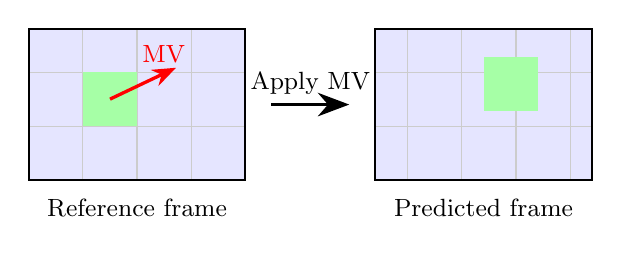
\begin{tikzpicture}[scale=0.55]
            % Reference frame
            \fill[blue!10] (0,0) rectangle (5,3.5);
            \draw[step=1.25, gray!40, thin] (0,0) grid (5,3.5);
            \fill[green!35] (1.25,1.25) rectangle (2.5,2.5);
            \draw[thick] (0,0) rectangle (5,3.5);
            \node[below,font=\small] at (2.5,-0.2) {Reference frame};
            
            % Motion vector arrow (clean, no overlap)
            \draw[-{Stealth[length=3mm]},red,very thick] (1.875,1.875) -- (3.4,2.6);
            \node[red,font=\small,above right] at (2.4,2.5) {MV};
            
            % Big arrow between frames
            \draw[-{Stealth[length=4mm]},thick] (5.6,1.75) -- (7.4,1.75)
                node[midway,above,font=\small] {Apply MV};
            
            % Predicted frame
            \fill[blue!10] (8,0) rectangle (13,3.5);
            \draw[step=1.25, gray!40, thin] (8,0) grid (13,3.5);
            \fill[green!35] (10.5,1.6) rectangle (11.75,2.85);
            \draw[thick] (8,0) rectangle (13,3.5);
            \node[below,font=\small] at (10.5,-0.2) {Predicted frame};
        \end{tikzpicture}
    \end{center}
\end{frame}

\begin{frame}{Block-Based Motion Estimation}
    \begin{columns}
        \begin{column}{0.55\textwidth}
            \textbf{How motion vectors are found:}
            \begin{enumerate}
                \item Divide current frame into blocks (16$\times$16)
                \item For each block, search the reference frame for the best match
                \item The displacement = motion vector
                \item Store: motion vector + residual error
            \end{enumerate}
            
            \vspace{0.3cm}
            \textbf{Search methods:}
            \begin{itemize}
                \item Full search (exhaustive, slow)
                \item Three-step search
                \item Diamond search
                \item Hierarchical search
            \end{itemize}
        \end{column}
        \begin{column}{0.4\textwidth}
            \begin{center}
                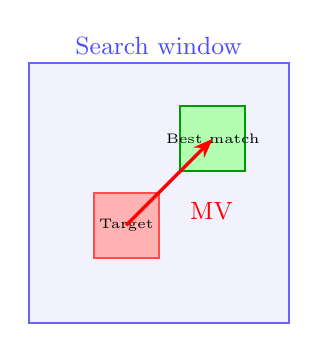
\begin{tikzpicture}[scale=0.55]
                    % Search area (outer)
                    \fill[blue!5] (0,0) rectangle (6,6);
                    \draw[thick, blue!60] (0,0) rectangle (6,6);
                    \node[blue!70,font=\small] at (3,6.4) {Search window};
                    
                    % Target block (lower-left area)
                    \fill[red!30] (1.5,1.5) rectangle (3,3);
                    \draw[thick,red!70] (1.5,1.5) rectangle (3,3);
                    \node[font=\tiny] at (2.25,2.25) {Target};
                    
                    % Best match (upper-right area, no overlap)
                    \fill[green!30] (3.5,3.5) rectangle (5,5);
                    \draw[thick,green!60!black] (3.5,3.5) rectangle (5,5);
                    \node[font=\tiny] at (4.25,4.25) {Best match};
                    
                    % Motion vector (clean diagonal)
                    \draw[-{Stealth[length=2.5mm]},red,very thick]
                        (2.25,2.25) -- (4.25,4.25);
                    \node[red,font=\small,below right] at (3.5,3) {MV};
                \end{tikzpicture}
            \end{center}
        \end{column}
    \end{columns}
\end{frame}


\begin{frame}{Motion Compensated Prediction: Encoder}
    \begin{center}
        \begin{tikzpicture}[
            xscale=0.95, yscale=0.85,
            every node/.style={font=\footnotesize},
            box/.style={draw, rounded corners=2pt, minimum width=1.4cm,
                minimum height=0.55cm, fill=##1, align=center},
            box/.default={blue!10},
            >=Stealth
        ]
            % === ROW 1 (y=4): forward path ===
            \node[box=yellow!20] (in)  at (0,4)   {Input};
            \node[draw,circle,fill=yellow!25,inner sep=1.5pt,font=\small] (sub) at (2,4) {$-$};
            \node[box]           (dct) at (4,4)   {DCT};
            \node[box=orange!15] (q)   at (6,4)   {Quant};
            \node[box=red!15]    (vlc) at (8,4)   {VLC};
            \node[box=gray!18]   (out) at (10,4)  {Bitstream};

            \draw[->,thick] (in) -- (sub);
            \draw[->,thick] (sub) -- (dct);
            \draw[->,thick] (dct) -- (q);
            \draw[->,thick] (q) -- (vlc);
            \draw[->,thick] (vlc) -- (out);

            % === ROW 2 (y=2): reconstruction ===
            \node[box]           (iq)   at (6,2)  {Inv Q};
            \node[box]           (idct) at (4,2)  {IDCT};
            \node[draw,circle,fill=yellow!25,inner sep=1.5pt,font=\small] (add) at (2,2) {$+$};

            \draw[->,thick] (q) -- (iq);
            \draw[->,thick] (iq) -- (idct);
            \draw[->,thick] (idct) -- (add);

            % === ROW 3 (y=0): motion + buffer ===
            \node[box=green!15]  (buf) at (2,0)   {Frame Buf};
            \node[box=green!18]  (mc)  at (5,0)   {Motion\\Comp};
            \node[box=red!15]    (me)  at (8,0)   {Motion\\Est};

            % add -> buf (straight down)
            \draw[->,thick] (add) -- (buf);

            % buf -> mc (straight right)
            \draw[->,thick] (buf) -- (mc);

            % buf -> me (below buf, then right)
            \draw[->,thick] (buf.south) -- ++(0,-0.5) -| (me.south);

            % me -> mc (straight left, above row 3)
            \draw[->,thick,red!60] (me.west) -- (mc.east)
                node[midway,above,font=\scriptsize]{MVs};

            % mc -> add (straight up)
            \draw[->,thick] (mc.north) -- ++(0,0.7) -| (add.south);

            % add -> sub (prediction, straight up)
            \draw[->,thick,densely dashed,blue!50] (add.north) -- (sub.south);

            % input -> me (left side down, then right along bottom)
            \draw[->,thick,gray] (in.south) -- ++(0,-1) -| (me.north);

            % me -> bitstream (go right past all boxes, then up, then left to out)
            \draw[->,thick,red!60] (me.east) -- (11,0) -- (11,4) -- (out.east)
                node[pos=0.25,right,font=\scriptsize]{MVs to bitstream};
        \end{tikzpicture}
    \end{center}
    
    \vspace{0.1cm}
    \small Subtract prediction $\to$ DCT $\to$ Quantize $\to$ VLC $\to$ Bitstream. Reconstruction loop rebuilds reference frames.
    
    \vspace{0.05cm}
    {\scriptsize DCT = Discrete Cosine Transform, VLC = Variable Length Coding, MV = Motion Vector}
\end{frame}

\begin{frame}{Frame Types: I, P, and B Frames}
    \begin{columns}
        \begin{column}{0.48\textwidth}
            \textbf{I-Frame (Intra):}
            \begin{itemize}
                \item Coded independently (like JPEG)
                \item No motion compensation
                \item Largest size, random access point
            \end{itemize}
            
            \vspace{0.15cm}
            \textbf{P-Frame (Predicted):}
            \begin{itemize}
                \item Predicted from previous I or P
                \item Forward prediction only
                \item Medium size
            \end{itemize}
            
            \vspace{0.15cm}
            \textbf{B-Frame (Bidirectional):}
            \begin{itemize}
                \item Predicted from past AND future
                \item Smallest size, best compression
            \end{itemize}
        \end{column}
        \begin{column}{0.48\textwidth}
            \begin{center}
                \begin{tikzpicture}[
                    scale=0.42,
                    fbox/.style={draw, minimum width=0.9cm, minimum height=1.4cm,
                        fill=##1, font=\small\bfseries}
                ]
                    % Frames on a line
                    \node[fbox=red!30]   (I)  at (0,0)  {I};
                    \node[fbox=blue!25]  (B1) at (2,0)  {B};
                    \node[fbox=blue!25]  (B2) at (4,0)  {B};
                    \node[fbox=green!30] (P1) at (6,0)  {P};
                    \node[fbox=blue!25]  (B3) at (8,0)  {B};
                    \node[fbox=blue!25]  (B4) at (10,0) {B};
                    \node[fbox=green!30] (P2) at (12,0) {P};

                    % Forward prediction (above, clean arcs)
                    \draw[-{Stealth},thick,red!70]
                        (I.north)  to[out=60,in=120] (P1.north);
                    \draw[-{Stealth},thick,green!60!black]
                        (P1.north) to[out=60,in=120] (P2.north);

                    % B1 references (below, separate arcs)
                    \draw[-{Stealth},thick,blue!60,densely dashed]
                        (I.south)  to[out=-40,in=-140] (B1.south);
                    \draw[-{Stealth},thick,blue!60,densely dashed]
                        (P1.south) to[out=-140,in=-40] (B1.south);

                    % B2 references (below, wider arcs)
                    \draw[-{Stealth},thick,blue!60,densely dashed]
                        (I.south)  to[out=-50,in=-160] (B2.south);
                    \draw[-{Stealth},thick,blue!60,densely dashed]
                        (P1.south) to[out=-160,in=-30] (B2.south);

                    % Label
                    \node[font=\small] at (6,-3) {GOP: I B B P B B P \ldots};
                \end{tikzpicture}
            \end{center}
        \end{column}
    \end{columns}
\end{frame}

\begin{frame}{Group of Pictures (GOP)}
    \begin{block}{Definition}
        A GOP is a sequence of frames starting with an I-frame, followed by P and B frames. It is the basic unit for random access.
    \end{block}
    
    \vspace{0.3cm}
    \begin{center}
        \begin{tikzpicture}[scale=0.42,
            fbox/.style={draw, minimum width=0.7cm, minimum height=0.9cm,
                fill=##1, font=\footnotesize}]
            \node[fbox=red!30]   at (0,0)    {I};
            \node[fbox=blue!20]  at (1.4,0)  {B};
            \node[fbox=blue!20]  at (2.8,0)  {B};
            \node[fbox=green!30] at (4.2,0)  {P};
            \node[fbox=blue!20]  at (5.6,0)  {B};
            \node[fbox=blue!20]  at (7,0)    {B};
            \node[fbox=green!30] at (8.4,0)  {P};
            \node[fbox=blue!20]  at (9.8,0)  {B};
            \node[fbox=blue!20]  at (11.2,0) {B};
            \node[fbox=green!30] at (12.6,0) {P};
            \node[fbox=red!30]   at (14,0)   {I};
            
            \draw[decorate, decoration={brace, amplitude=6pt, raise=4pt}]
                (-0.5,0.7) -- (13.5,0.7)
                node[midway, above=10pt, font=\small] {One GOP ($N$=12, $M$=3)};
        \end{tikzpicture}
    \end{center}
    
    \vspace{0.3cm}
    \textbf{GOP parameters:}
    \begin{itemize}
        \item $N$ = GOP length (distance between I-frames), typically 12--15
        \item $M$ = distance between anchor frames (I or P), typically 3
        \item Larger $N$ $\rightarrow$ better compression, slower random access
    \end{itemize}
\end{frame}

\begin{frame}{Typical Compression Ratios}
    \begin{center}
        \begin{tabular}{l|c|c}
            \toprule
            \textbf{Frame Type} & \textbf{Typical Size} & \textbf{Compression} \\
            \midrule
            I-Frame & 150 KB & 10:1 \\
            P-Frame & 50 KB & 30:1 \\
            B-Frame & 20 KB & 75:1 \\
            \bottomrule
        \end{tabular}
    \end{center}
    
    \vspace{0.3cm}
    \textbf{Why B-frames compress best:}
    \begin{itemize}
        \item Bidirectional prediction is more accurate
        \item Smaller residual $\rightarrow$ fewer bits
        \item Interpolation between past and future works well
    \end{itemize}
    
    \vspace{0.3cm}
    \begin{alertblock}{Tradeoff}
        B-frames add encoding delay (need future frames) and complexity, but significantly improve compression.
    \end{alertblock}
\end{frame}


%==============================================================================
\section{MPEG-1: Video Bitstream}
%==============================================================================

\begin{frame}{What is MPEG?}
    \begin{block}{MPEG = Moving Picture Experts Group}
        A working group of ISO/IEC that develops standards for coded representation of digital audio and video. Established in 1988.
    \end{block}
    
    \vspace{0.3cm}
    \textbf{The MPEG family:}
    \begin{center}
        \begin{tabular}{l|c|l}
            \toprule
            \textbf{Standard} & \textbf{Year} & \textbf{Target Application} \\
            \midrule
            MPEG-1 & 1993 & CD-ROM video (VCD) \\
            MPEG-2 & 1995 & Broadcast TV, DVD \\
            MPEG-4 & 1999 & Internet, mobile \\
            MPEG-7 & 2002 & Content description \\
            \bottomrule
        \end{tabular}
    \end{center}
\end{frame}

\begin{frame}{MPEG-1: Overview}
    \textbf{Target:} Video and audio on CD-ROM at 1.5 Mbps
    
    \vspace{0.3cm}
    \textbf{Key specifications:}
    \begin{itemize}
        \item Resolution: 352$\times$240 (SIF --- Source Input Format)
        \item Frame rate: 30 fps (NTSC) or 25 fps (PAL)
        \item Progressive scan only (no interlacing)
        \item Total bitrate: $\sim$1.5 Mbps (1.15 video + 0.22 audio)
        \item Quality: comparable to VHS
    \end{itemize}
    
    \vspace{0.3cm}
    \begin{block}{Key Application}
        \textbf{VCD (Video CD)} --- the first widely used digital video format. Very popular in Asia in the 1990s.
    \end{block}
\end{frame}

\begin{frame}{MPEG-1 Video Bitstream Hierarchy}
    \begin{center}
        \begin{tikzpicture}[
            scale=0.52, every node/.style={scale=0.72},
            lbox/.style={draw, rounded corners=3pt, minimum width=3.2cm,
                minimum height=0.75cm, fill=##1, font=\small}
        ]
            \node[lbox=red!20]    (seq)   at (0,10) {\textbf{Video Sequence}};
            \node[lbox=orange!20] (gop)   at (0,8)  {\textbf{Group of Pictures}};
            \node[lbox=yellow!20] (pic)   at (0,6)  {\textbf{Picture (Frame)}};
            \node[lbox=green!20]  (slice) at (0,4)  {\textbf{Slice}};
            \node[lbox=blue!20]   (mb)    at (0,2)  {\textbf{Macroblock (16$\times$16)}};
            \node[lbox=purple!20] (blk)   at (0,0)  {\textbf{Block (8$\times$8)}};

            \draw[-{Stealth},thick] (seq)   -- (gop);
            \draw[-{Stealth},thick] (gop)   -- (pic);
            \draw[-{Stealth},thick] (pic)   -- (slice);
            \draw[-{Stealth},thick] (slice) -- (mb);
            \draw[-{Stealth},thick] (mb)    -- (blk);

            % Right-side descriptions (well separated)
            \node[right, font=\small, text=gray!70!black] at (2.5,10) {Header + sequence of GOPs};
            \node[right, font=\small, text=gray!70!black] at (2.5,8)  {I B B P B B P \ldots};
            \node[right, font=\small, text=gray!70!black] at (2.5,6)  {I-picture, P-picture, or B-picture};
            \node[right, font=\small, text=gray!70!black] at (2.5,4)  {One row of macroblocks};
            \node[right, font=\small, text=gray!70!black] at (2.5,2)  {4Y + 1Cb + 1Cr = 6 blocks};
            \node[right, font=\small, text=gray!70!black] at (2.5,0)  {DCT $\rightarrow$ Quantize $\rightarrow$ VLC};
        \end{tikzpicture}
    \end{center}
\end{frame}

\begin{frame}{Macroblock Structure (4:2:0)}
    \begin{columns}
        \begin{column}{0.5\textwidth}
            \begin{center}
                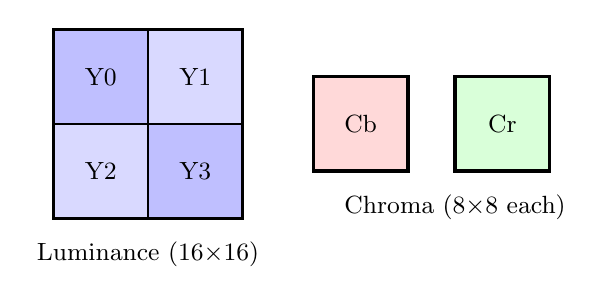
\begin{tikzpicture}[scale=0.6]
                    % 4 Y blocks
                    \fill[blue!15] (0,0) rectangle (2,2);
                    \fill[blue!25] (2,0) rectangle (4,2);
                    \fill[blue!25] (0,2) rectangle (2,4);
                    \fill[blue!15] (2,2) rectangle (4,4);
                    \draw[thick] (0,0) grid[step=2] (4,4);
                    \draw[very thick] (0,0) rectangle (4,4);
                    \node[font=\small] at (1,3) {Y0};
                    \node[font=\small] at (3,3) {Y1};
                    \node[font=\small] at (1,1) {Y2};
                    \node[font=\small] at (3,1) {Y3};
                    \node[below,font=\small] at (2,-0.3) {Luminance (16$\times$16)};
                    
                    % Cb
                    \fill[red!15] (5.5,1) rectangle (7.5,3);
                    \draw[very thick] (5.5,1) rectangle (7.5,3);
                    \node[font=\small] at (6.5,2) {Cb};
                    
                    % Cr
                    \fill[green!15] (8.5,1) rectangle (10.5,3);
                    \draw[very thick] (8.5,1) rectangle (10.5,3);
                    \node[font=\small] at (9.5,2) {Cr};
                    
                    \node[below,font=\small] at (8.5,0.7) {Chroma (8$\times$8 each)};
                \end{tikzpicture}
            \end{center}
        \end{column}
        \begin{column}{0.45\textwidth}
            \textbf{4:2:0 subsampling:}
            \begin{itemize}
                \item 4 luminance blocks (Y)
                \item 1 Cb chrominance block
                \item 1 Cr chrominance block
                \item Total: 6 blocks per macroblock
            \end{itemize}
            
            \vspace{0.3cm}
            \textbf{Each 8$\times$8 block:}
            \begin{itemize}
                \item DCT transformed
                \item Quantized
                \item Zigzag scanned
                \item Entropy coded (VLC --- Variable Length Coding)
            \end{itemize}
        \end{column}
    \end{columns}
\end{frame}

\begin{frame}{MPEG-1 Encoding Pipeline}
    \begin{center}
        \begin{tikzpicture}[
            xscale=0.95, yscale=0.85,
            every node/.style={font=\footnotesize},
            box/.style={draw, rounded corners=2pt, minimum width=1.3cm,
                minimum height=0.55cm, fill=##1, align=center},
            box/.default={blue!10},
            >=Stealth
        ]
            % === ROW 1 (y=3): forward path ===
            \node[box=yellow!20] (in)  at (0,3)   {Input};
            \node[box]           (sub) at (2,3)    {Subtract};
            \node[box]           (dct) at (4,3)    {DCT};
            \node[box=orange!15] (q)   at (6,3)    {Quant};
            \node[box=red!15]    (vlc) at (8,3)    {VLC};
            \node[box=gray!18]   (mux) at (10,3)   {Mux};

            \draw[->,thick] (in) -- (sub);
            \draw[->,thick] (sub) -- (dct);
            \draw[->,thick] (dct) -- (q);
            \draw[->,thick] (q) -- (vlc);
            \draw[->,thick] (vlc) -- (mux);

            % === ROW 2 (y=1.2): reconstruction ===
            \node[box]           (iq)   at (6,1.2)  {Inv Q};
            \node[box]           (idct) at (4,1.2)  {IDCT};
            \node[box=green!15]  (mc)   at (2,1.2)  {MC Pred};

            \draw[->,thick] (q) -- (iq);
            \draw[->,thick] (iq) -- (idct);
            \draw[->,thick] (idct) -- (mc);
            \draw[->,thick] (mc.north) -- (sub.south);

            % === ROW 3 (y=-0.5): buffer + ME ===
            \node[box=green!15]  (buf) at (2,-0.5)  {Frame Buf};
            \node[box=red!15]    (me)  at (6,-0.5)  {Motion Est};

            \draw[->,thick] (mc) -- (buf);
            \draw[->,thick] (buf) -- (me);

            % ME -> Mux (motion vectors, right side path)
            \draw[->,thick,red!60] (me.east) -| (10,1.2) -- (mux.south);

            % Input -> ME (left side path, no crossing)
            \draw[->,thick,gray] (in.south) -- ++(0,-0.8) -| (me.north);

            % ME -> MC (motion vectors back)
            \draw[->,thick,red!60] (me.north west) -- ++(0,0.5) -| (mc.south);

            \node[right,font=\scriptsize] at (10.5,3) {Bitstream};
        \end{tikzpicture}
    \end{center}
    
    \vspace{0.1cm}
    \small\textbf{Steps:} Input $\rightarrow$ Subtract prediction $\rightarrow$ DCT $\rightarrow$ Quantize $\rightarrow$ VLC $\rightarrow$ Bitstream.
    
    {\scriptsize VLC = Variable Length Coding, MC = Motion Compensated, IDCT = Inverse DCT}
\end{frame}

\begin{frame}{MPEG-1 Decoding Pipeline}
    \begin{center}
        \begin{tikzpicture}[
            xscale=1.05, yscale=0.9,
            every node/.style={font=\footnotesize},
            box/.style={draw, rounded corners=2pt, minimum width=1.5cm,
                minimum height=0.55cm, fill=##1, align=center},
            box/.default={blue!10},
            >=Stealth
        ]
            % === ROW 1 (y=2.5): forward decode path ===
            \node[box=gray!18]   (in)   at (0,2.5)   {Bitstream};
            \node[box=red!15]    (vld)  at (2.5,2.5)  {VLD};
            \node[box=orange!15] (iq)   at (5,2.5)    {Inv Quant};
            \node[box]           (idct) at (7.5,2.5)  {IDCT};
            \node[draw,circle,fill=yellow!25,inner sep=1.5pt,font=\small]
                                 (add)  at (9.5,2.5)  {$+$};
            \node[box=green!18]  (out)  at (11.5,2.5) {Output\\Frame};

            \draw[->,thick] (in) -- (vld);
            \draw[->,thick] (vld) -- (iq);
            \draw[->,thick] (iq) -- (idct);
            \draw[->,thick] (idct) -- (add);
            \draw[->,thick] (add) -- (out);

            % === ROW 2 (y=0.5): motion compensation ===
            \node[box=green!15]  (buf) at (9.5,0.5)  {Frame Buf};
            \node[box=green!18]  (mc)  at (5,0.5)    {Motion\\Comp};

            % add -> buffer
            \draw[->,thick] (add) -- (buf);

            % buffer -> mc
            \draw[->,thick] (buf) -- (mc);

            % mc -> add (prediction fed back)
            \draw[->,thick] (mc.north) -- ++(0,0.7) -| (add.south);

            % VLD sends MVs to MC (clean path below)
            \draw[->,thick,red!60] (vld.south) -- ++(0,-0.5) -| (mc.north)
                node[pos=0.3,right,font=\scriptsize]{MVs};
        \end{tikzpicture}
    \end{center}

    \vspace{0.1cm}
    \small\textbf{Decoder is much simpler than encoder:} No motion estimation needed! Just apply the motion vectors received in the bitstream.

    {\scriptsize VLD = Variable Length Decoding (inverse of VLC)}
\end{frame}


%==============================================================================
\section{MPEG-2: Supporting Interlaced Video}
%==============================================================================

\begin{frame}{MPEG-2: Why a New Standard?}
    \textbf{MPEG-1 limitations:}
    \begin{itemize}
        \item Low resolution only (352$\times$240)
        \item No interlaced video support
        \item No scalability (one quality level)
        \item Not suitable for broadcast TV
    \end{itemize}
    
    \vspace{0.3cm}
    \begin{block}{MPEG-2 Goals}
        \begin{itemize}
            \item Support broadcast-quality video (720$\times$480 and above)
            \item Handle \textbf{interlaced} video (standard for TV)
            \item Provide \textbf{scalable} coding (multiple quality layers)
            \item Bitrates from 2 to 80 Mbps
        \end{itemize}
    \end{block}
    
    \vspace{0.2cm}
    \textbf{Applications:} DVD, Digital TV (DVB), HDTV, Satellite broadcasting
\end{frame}

\begin{frame}{Interlaced vs Progressive Video}
    \begin{columns}
        \begin{column}{0.48\textwidth}
            \textbf{Progressive (MPEG-1):}
            \begin{center}
                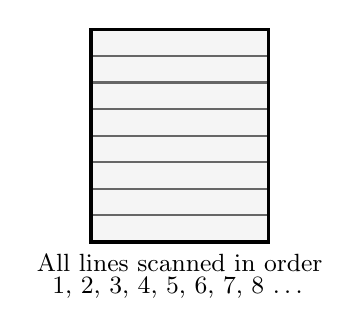
\begin{tikzpicture}[scale=0.45]
                    \fill[gray!8] (0,0) rectangle (5,6);
                    \foreach \y in {0,...,7} {
                        \draw[black!60, thick] (0,\y*0.75) -- (5,\y*0.75);
                    }
                    \draw[very thick] (0,0) rectangle (5,6);
                    \node[font=\small] at (2.5,-0.6) {All lines scanned in order};
                    \node[font=\small] at (2.5,-1.3) {1, 2, 3, 4, 5, 6, 7, 8 \ldots};
                \end{tikzpicture}
            \end{center}
            
            Used in computer monitors and modern displays.
        \end{column}
        \begin{column}{0.48\textwidth}
            \textbf{Interlaced (MPEG-2):}
            \begin{center}
                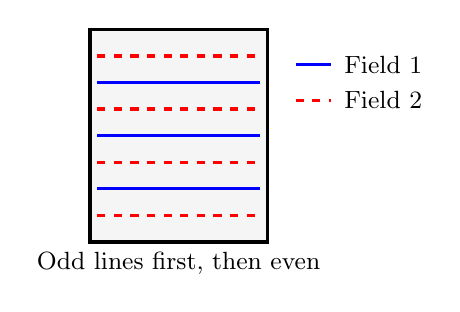
\begin{tikzpicture}[scale=0.45]
                    \fill[gray!8] (0,0) rectangle (5,6);
                    % Odd field (solid blue lines)
                    \foreach \y in {0,1.5,3,4.5} {
                        \draw[blue, line width=1.2pt] (0.2,\y) -- (4.8,\y);
                    }
                    % Even field (dashed red lines, offset)
                    \foreach \y in {0.75,2.25,3.75,5.25} {
                        \draw[red, line width=1.2pt, dashed] (0.2,\y) -- (4.8,\y);
                    }
                    \draw[very thick] (0,0) rectangle (5,6);
                    % Legend outside the frame
                    \draw[blue, line width=1.2pt] (5.8,5) -- (6.8,5);
                    \node[right,font=\small] at (6.9,5) {Field 1};
                    \draw[red, line width=1.2pt, dashed] (5.8,4) -- (6.8,4);
                    \node[right,font=\small] at (6.9,4) {Field 2};
                    \node[font=\small] at (2.5,-0.6) {Odd lines first, then even};
                \end{tikzpicture}
            \end{center}
            
            Each frame = 2 fields. Standard for analog and early digital TV.
        \end{column}
    \end{columns}
\end{frame}

\begin{frame}{MPEG-2 Interlaced Coding Modes}
    \textbf{MPEG-2 supports two coding modes for interlaced video:}
    
    \vspace{0.3cm}
    \begin{columns}
        \begin{column}{0.48\textwidth}
            \textbf{Frame Picture:}
            \begin{itemize}
                \item Both fields merged into one frame
                \item Good for slow-moving scenes
                \item Better spatial correlation
            \end{itemize}
            
            \begin{center}
                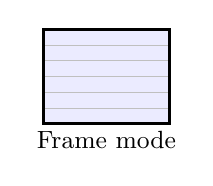
\begin{tikzpicture}[scale=0.4]
                    \fill[blue!8] (0,0) rectangle (4,3);
                    \foreach \y in {0,...,5} {
                        \draw[gray!50] (0,\y*0.5) -- (4,\y*0.5);
                    }
                    \draw[very thick] (0,0) rectangle (4,3);
                    \node[font=\small] at (2,-0.5) {Frame mode};
                \end{tikzpicture}
            \end{center}
        \end{column}
        \begin{column}{0.48\textwidth}
            \textbf{Field Picture:}
            \begin{itemize}
                \item Each field coded separately
                \item Good for fast-moving scenes
                \item Better temporal correlation
            \end{itemize}
            
            \begin{center}
                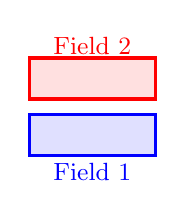
\begin{tikzpicture}[scale=0.4]
                    \fill[blue!12] (0,0) rectangle (4,1.3);
                    \draw[very thick, blue] (0,0) rectangle (4,1.3);
                    \node[blue,font=\small] at (2,-0.5) {Field 1};
                    
                    \fill[red!12] (0,1.8) rectangle (4,3.1);
                    \draw[very thick, red] (0,1.8) rectangle (4,3.1);
                    \node[red,font=\small] at (2,3.5) {Field 2};
                \end{tikzpicture}
            \end{center}
        \end{column}
    \end{columns}
    
    \vspace{0.3cm}
    \textit{The encoder chooses the best mode for each macroblock adaptively.}
\end{frame}

\begin{frame}{MPEG-2 Profiles and Levels}
    \textbf{MPEG-2 uses Profiles (features) $\times$ Levels (resolution):}
    
    \vspace{0.3cm}
    \begin{center}
        \small
        \begin{tabular}{l|c|c|c}
            \toprule
            & \textbf{Simple} & \textbf{Main} & \textbf{High} \\
            \midrule
            \textbf{Low} (352$\times$288) & --- & 4 Mbps & --- \\
            \textbf{Main} (720$\times$576) & 15 Mbps & 15 Mbps & 20 Mbps \\
            \textbf{High-1440} & --- & 60 Mbps & 80 Mbps \\
            \textbf{High} (1920$\times$1080) & --- & 80 Mbps & 100 Mbps \\
            \bottomrule
        \end{tabular}
    \end{center}
    
    \vspace{0.3cm}
    \textbf{Most common:} Main Profile @ Main Level (MP@ML)
    \begin{itemize}
        \item Used in DVD and standard digital TV
        \item 720$\times$576 resolution, up to 15 Mbps
        \item Supports I, P, B frames
    \end{itemize}
\end{frame}

\begin{frame}{MPEG-2 Scalability}
    \textbf{MPEG-2 introduces scalable coding --- multiple quality layers:}
    
    \vspace{0.3cm}
    \begin{columns}
        \begin{column}{0.48\textwidth}
            \textbf{SNR Scalability:}
            \begin{itemize}
                \item Base layer: low quality
                \item Enhancement: adds detail
                \item Same resolution, better quality
            \end{itemize}
            
            \vspace{0.2cm}
            \textbf{Spatial Scalability:}
            \begin{itemize}
                \item Base layer: low resolution
                \item Enhancement: higher resolution
                \item e.g., SD base + HD enhancement
            \end{itemize}
        \end{column}
        \begin{column}{0.48\textwidth}
            \textbf{Temporal Scalability:}
            \begin{itemize}
                \item Base layer: low frame rate
                \item Enhancement: more frames
                \item e.g., 15 fps base + 30 fps full
            \end{itemize}
            
            \vspace{0.3cm}
            \begin{block}{Why Scalability?}
                Different receivers decode different layers based on capability and bandwidth.
            \end{block}
        \end{column}
    \end{columns}
\end{frame}

\begin{frame}{MPEG-1 vs MPEG-2 Comparison}
    \begin{center}
        \begin{tabular}{l|c|c}
            \toprule
            \textbf{Feature} & \textbf{MPEG-1} & \textbf{MPEG-2} \\
            \midrule
            Year & 1993 & 1995 \\
            Resolution & Up to SIF & Up to HDTV \\
            Scan type & Progressive only & Progressive + Interlaced \\
            Bitrate & 1.5 Mbps & 2--80 Mbps \\
            Scalability & No & Yes (SNR, spatial, temporal) \\
            Profiles/Levels & No & Yes \\
            Application & VCD & DVD, Digital TV, HDTV \\
            \bottomrule
        \end{tabular}
    \end{center}
    
    \vspace{0.3cm}
    \textbf{MPEG-2 is a superset of MPEG-1.} An MPEG-2 decoder can decode MPEG-1 streams.
\end{frame}


%==============================================================================
\section{MPEG-4: Overview}
%==============================================================================

\begin{frame}{MPEG-4: A New Paradigm}
    \textbf{MPEG-1/2 treat video as rectangular frames.}
    
    \textbf{MPEG-4 treats video as a collection of \textit{objects}.}
    
    \vspace{0.3cm}
    \begin{block}{MPEG-4 Vision}
        A scene is composed of audio-visual objects that can be independently coded, transmitted, and manipulated.
    \end{block}
    
    \vspace{0.3cm}
    \textbf{Target applications:}
    \begin{itemize}
        \item Internet video streaming (low bitrate)
        \item Mobile multimedia
        \item Interactive TV and content-based retrieval
        \item Very low bitrate (8--64 kbps) to high bitrate
    \end{itemize}
\end{frame}

\begin{frame}{MPEG-4: Object-Based Coding}
    \begin{center}
        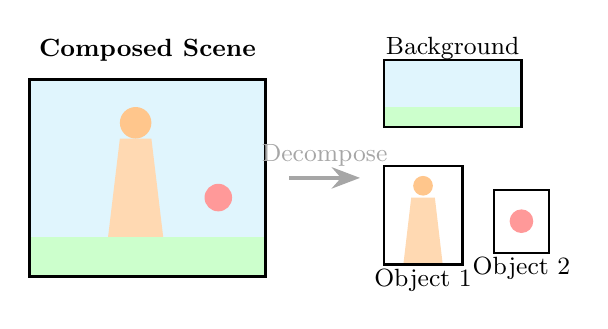
\begin{tikzpicture}[scale=0.5, >=Stealth]
            % --- Left: Composed scene ---
            \fill[cyan!12] (0,0) rectangle (6,5);
            \fill[green!20] (0,0) rectangle (6,1);
            \draw[very thick] (0,0) rectangle (6,5);

            % Person (clean trapezoid + circle head)
            \fill[orange!30] (2,1) -- (2.3,3.5) -- (3.1,3.5) -- (3.4,1) -- cycle;
            \fill[orange!45] (2.7,3.9) circle (0.4);

            % Ball (clean circle, well separated)
            \fill[red!40] (4.8,2) circle (0.35);

            \node[above,font=\small\bfseries] at (3,5.2) {Composed Scene};

            % Arrow
            \draw[->,ultra thick,gray!70] (6.6,2.5) -- (8.4,2.5)
                node[midway,above,font=\small] {Decompose};

            % --- Right: Three separate boxes ---
            % Background (top right)
            \fill[cyan!12] (9,3.8) rectangle (12.5,5.5);
            \fill[green!20] (9,3.8) rectangle (12.5,4.3);
            \draw[thick] (9,3.8) rectangle (12.5,5.5);
            \node[font=\small] at (10.75,5.8) {Background};

            % Person object (bottom left)
            \fill[white] (9,0.3) rectangle (11,2.8);
            \fill[orange!30] (9.5,0.3) -- (9.7,2) -- (10.3,2) -- (10.5,0.3) -- cycle;
            \fill[orange!45] (10,2.3) circle (0.25);
            \draw[thick] (9,0.3) rectangle (11,2.8);
            \node[font=\small] at (10,-0.1) {Object 1};

            % Ball object (bottom right)
            \fill[white] (11.8,0.6) rectangle (13.2,2.2);
            \fill[red!40] (12.5,1.4) circle (0.3);
            \draw[thick] (11.8,0.6) rectangle (13.2,2.2);
            \node[font=\small] at (12.5,0.2) {Object 2};
        \end{tikzpicture}
    \end{center}

    \vspace{0.2cm}
    Each object is coded, transmitted, and decoded independently. The decoder composes them back into a scene.
\end{frame}

\begin{frame}{MPEG-4 Video Object Plane (VOP)}
    \begin{columns}
        \begin{column}{0.5\textwidth}
            \textbf{Key concepts:}
            \begin{itemize}
                \item \textbf{VO} (Video Object): A semantic entity (person, car, background)
                \item \textbf{VOP} (Video Object Plane): One instance of a VO at a specific time
                \item \textbf{VOL} (Video Object Layer): Scalable representation of a VO
            \end{itemize}
            
            \vspace{0.2cm}
            \textbf{VOP types} (same idea as frames):
            \begin{itemize}
                \item I-VOP, P-VOP, B-VOP
            \end{itemize}
        \end{column}
        \begin{column}{0.45\textwidth}
            \begin{center}
                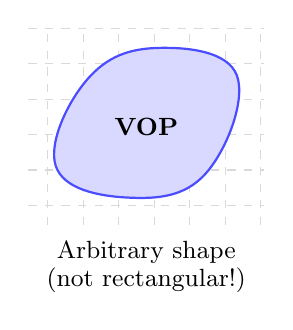
\begin{tikzpicture}[scale=0.5]
                    % Dashed grid (background, drawn first)
                    \draw[step=0.9, gray!30, thin, dashed] (-0.5,-0.5) grid (5.5,4.5);
                    
                    % Arbitrary shape (drawn on top of grid)
                    \fill[blue!15]
                        plot[smooth cycle, tension=0.7]
                        coordinates {(0.2,1) (1,3.2) (2.8,4) (4.8,3.3) (4,0.8) (2,0.2)};
                    \draw[thick, blue!70]
                        plot[smooth cycle, tension=0.7]
                        coordinates {(0.2,1) (1,3.2) (2.8,4) (4.8,3.3) (4,0.8) (2,0.2)};
                    
                    \node[font=\small\bfseries] at (2.5,2) {VOP};
                    \node[font=\small] at (2.5,-1.2) {Arbitrary shape};
                    \node[font=\small] at (2.5,-1.9) {(not rectangular!)};
                \end{tikzpicture}
            \end{center}
        \end{column}
    \end{columns}
\end{frame}

\begin{frame}{MPEG-4 Scene Composition (BIFS)}
    \begin{block}{BIFS = Binary Format for Scenes}
        Describes how audio-visual objects are composed into a scene. Based on VRML.
    \end{block}
    
    \vspace{0.3cm}
    \begin{center}
        \begin{tikzpicture}[
            scale=0.55, every node/.style={scale=0.72},
            sbox/.style={draw, rounded corners=3pt, minimum width=2.2cm,
                minimum height=0.7cm, fill=##1, font=\small}
        ]
            \node[sbox=red!20] (scene) at (5,5) {\textbf{Scene (BIFS)}};
            
            \node[sbox=blue!15]   (bg)  at (1,3)  {Background};
            \node[sbox=green!15]  (vid) at (5,3)  {Video Object};
            \node[sbox=orange!15] (aud) at (9,3)  {Audio Object};
            \node[sbox=purple!15] (txt) at (5,1)  {Text / Graphics};
            
            \draw[-{Stealth},thick] (scene) -- (bg);
            \draw[-{Stealth},thick] (scene) -- (vid);
            \draw[-{Stealth},thick] (scene) -- (aud);
            \draw[-{Stealth},thick] (scene) -- (txt);
        \end{tikzpicture}
    \end{center}
    
    \vspace{0.2cm}
    BIFS specifies position, size, timing, and interaction behavior of each object in the scene.
\end{frame}

\begin{frame}{MPEG-4 Parts}
    \textbf{MPEG-4 is a large standard with many parts:}
    
    \vspace{0.3cm}
    \begin{center}
        \small
        \begin{tabular}{c|l|l}
            \toprule
            \textbf{Part} & \textbf{Name} & \textbf{Description} \\
            \midrule
            Part 1 & Systems & Scene description, sync \\
            Part 2 & Visual & Video coding (incl.\ shape) \\
            Part 3 & Audio & Audio coding (AAC) \\
            Part 10 & AVC (H.264) & Advanced Video Coding \\
            Part 12 & File Format & ISO base media file \\
            Part 14 & MP4 File & .mp4 container format \\
            \bottomrule
        \end{tabular}
    \end{center}
    
    \vspace{0.3cm}
    \begin{alertblock}{Most Important}
        \textbf{MPEG-4 Part 10 (H.264/AVC)} became the dominant video codec for the internet, Blu-ray, and mobile video.
    \end{alertblock}
\end{frame}

\begin{frame}{MPEG-4 vs MPEG-1/2}
    \begin{center}
        \begin{tabular}{l|c|c|c}
            \toprule
            \textbf{Feature} & \textbf{MPEG-1} & \textbf{MPEG-2} & \textbf{MPEG-4} \\
            \midrule
            Coding unit & Frame & Frame/Field & Object \\
            Shape coding & No & No & Yes \\
            Scalability & No & Yes & Yes \\
            Interactivity & No & No & Yes \\
            Bitrate range & 1.5 Mbps & 2--80 Mbps & 8 kbps+ \\
            Sprite coding & No & No & Yes \\
            Error resilience & Basic & Basic & Advanced \\
            \bottomrule
        \end{tabular}
    \end{center}
    
    \vspace{0.3cm}
    \textbf{MPEG-4 key innovations:}
    \begin{itemize}
        \item Object-based coding with arbitrary shapes
        \item Very low bitrate coding for mobile
        \item Content-based interactivity and sprite coding
    \end{itemize}
\end{frame}


%==============================================================================
\section{MPEG-7: Introduction}
%==============================================================================

\begin{frame}{MPEG-7: Not a Codec!}
    \begin{alertblock}{Important Distinction}
        MPEG-7 is \textbf{NOT} a compression standard. It does not code audio or video. It \textbf{describes} multimedia content.
    \end{alertblock}
    
    \vspace{0.3cm}
    \begin{block}{MPEG-7 = Multimedia Content Description Interface (2002)}
        A standard for describing multimedia content, enabling efficient searching, filtering, and browsing of audio-visual material.
    \end{block}
    
    \vspace{0.3cm}
    \textbf{Analogy:}
    \begin{itemize}
        \item MPEG-1/2/4 = the \textbf{book} (content itself)
        \item MPEG-7 = the \textbf{library catalog} (description of content)
    \end{itemize}
\end{frame}

\begin{frame}{Why MPEG-7?}
    \begin{columns}
        \begin{column}{0.5\textwidth}
            \textbf{Text search is easy:}
            \begin{itemize}
                \item Search for ``sunset beach''
                \item Match keywords in documents
            \end{itemize}
            
            \vspace{0.2cm}
            \textbf{Multimedia search is hard:}
            \begin{itemize}
                \item Find a photo with a red car
                \item Find music that sounds like X
                \item Find a video scene with a dog
            \end{itemize}
        \end{column}
        \begin{column}{0.45\textwidth}
            \begin{block}{MPEG-7 Solution}
                Attach standardized descriptions:
                \begin{itemize}
                    \item Colors in the image
                    \item Textures and shapes
                    \item Sounds and melody
                    \item Who, when, where
                \end{itemize}
            \end{block}
        \end{column}
    \end{columns}
\end{frame}

\begin{frame}{MPEG-7 Architecture}
    \begin{center}
        \begin{tikzpicture}[
            scale=0.58, every node/.style={scale=0.72},
            abox/.style={draw, rounded corners=3pt, minimum width=3.5cm,
                minimum height=0.8cm, fill=##1, font=\small}
        ]
            % Top: DDL
            \node[abox=red!18] (ddl) at (5,6) {\textbf{DDL} (Description Definition Language)};
            
            % Middle row
            \node[abox=blue!18]  (d)  at (2,3.5) {\textbf{Descriptors} (D)};
            \node[abox=green!18] (ds) at (8,3.5) {\textbf{Description Schemes} (DS)};
            
            % Bottom row
            \node[abox=orange!18] (sys) at (2,1) {System Tools};
            \node[abox=purple!18] (ref) at (8,1) {Reference Software};
            
            % Arrows (clean, no crossing)
            \draw[-{Stealth},thick] (ddl.south west) -- (d.north);
            \draw[-{Stealth},thick] (ddl.south east) -- (ds.north);
            \draw[-{Stealth},thick] (d) -- (sys);
            \draw[-{Stealth},thick] (ds) -- (ref);
            
            % Side labels
            \node[left, font=\small, text=gray!60!black] at (-0.5,3.5) {Low-level features};
            \node[right, font=\small, text=gray!60!black] at (10.5,3.5) {Structures of D's};
            \node[right, font=\small, text=gray!60!black] at (10.5,6) {XML-based};
        \end{tikzpicture}
    \end{center}
    
    \vspace{0.3cm}
    \textbf{Three main components:}
    \begin{itemize}
        \item \textbf{Descriptors (D):} Represent a feature (color, texture, shape, motion)
        \item \textbf{Description Schemes (DS):} Structure that combines descriptors
        \item \textbf{DDL:} XML-based language to define D's and DS's
    \end{itemize}
\end{frame}

\begin{frame}{MPEG-7 Visual Descriptors}
    \begin{columns}
        \begin{column}{0.48\textwidth}
            \textbf{Color Descriptors:}
            \begin{itemize}
                \item Dominant Color
                \item Color Layout
                \item Color Structure
                \item Scalable Color (histogram)
            \end{itemize}
            
            \vspace{0.2cm}
            \textbf{Texture Descriptors:}
            \begin{itemize}
                \item Homogeneous Texture
                \item Edge Histogram
                \item Texture Browsing
            \end{itemize}
        \end{column}
        \begin{column}{0.48\textwidth}
            \textbf{Shape Descriptors:}
            \begin{itemize}
                \item Region Shape
                \item Contour Shape
                \item 3D Shape
            \end{itemize}
            
            \vspace{0.2cm}
            \textbf{Motion Descriptors:}
            \begin{itemize}
                \item Camera Motion
                \item Motion Trajectory
                \item Motion Activity
                \item Parametric Motion
            \end{itemize}
        \end{column}
    \end{columns}
\end{frame}

\begin{frame}{MPEG-7 Audio Descriptors}
    \begin{columns}
        \begin{column}{0.48\textwidth}
            \textbf{Low-level:}
            \begin{itemize}
                \item Audio Waveform
                \item Audio Power
                \item Audio Spectrum Envelope
                \item Audio Fundamental Frequency
                \item Audio Harmonicity
            \end{itemize}
        \end{column}
        \begin{column}{0.48\textwidth}
            \textbf{High-level:}
            \begin{itemize}
                \item Sound Classification
                \item Musical Instrument Timbre
                \item Melody Description
                \item Spoken Content
            \end{itemize}
            
            \vspace{0.3cm}
            \begin{block}{Example Use}
                ``Find songs with similar melody to this hummed tune''
            \end{block}
        \end{column}
    \end{columns}
\end{frame}

\begin{frame}{MPEG-7 Example: Content-Based Image Retrieval}
    \begin{center}
        \begin{tikzpicture}[
            xscale=1.1, yscale=0.9,
            every node/.style={font=\footnotesize},
            rbox/.style={draw, rounded corners=2pt, minimum width=2cm,
                minimum height=0.7cm, fill=##1, align=center},
            >=Stealth
        ]
            % Top row: query path (left to right)
            \node[rbox=yellow!20] (query) at (0,3)   {Query Image};
            \node[rbox=blue!12]   (feat)  at (3,3)   {Extract\\Descriptors};
            \node[rbox=green!12]  (qdesc) at (6,3)   {MPEG-7\\Description};

            \draw[->,thick] (query) -- (feat);
            \draw[->,thick] (feat)  -- (qdesc);

            % Bottom left: database
            \node[rbox=orange!15, minimum height=1.2cm] (db) at (3,0.5) {MPEG-7\\Database};

            % Bottom right: match + results
            \node[rbox=red!15]    (match) at (6,0.5)  {Match \&\\Rank};
            \node[rbox=purple!15] (res)   at (9,0.5)  {Similar\\Images};

            % Arrows: qdesc down to match (vertical then horizontal)
            \draw[->,thick] (qdesc.south) -- (match.north);

            % db to match (straight right)
            \draw[->,thick] (db) -- (match);

            % match to results (straight right)
            \draw[->,thick] (match) -- (res);
        \end{tikzpicture}
    \end{center}

    \vspace{0.2cm}
    \textbf{Process:} Extract descriptors from query $\to$ Compare with database $\to$ Return most similar results.
\end{frame}

\begin{frame}{The Complete MPEG Family Timeline}
    \begin{center}
        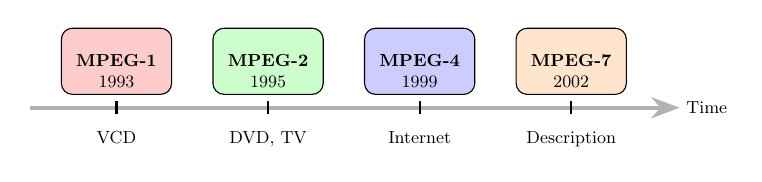
\begin{tikzpicture}[scale=0.55, every node/.style={scale=0.7}]
            % Timeline
            \draw[-{Stealth},ultra thick, gray!60] (0,0) -- (15,0);
            \node[right,font=\small] at (15,0) {Time};
            
            % MPEG-1
            \draw[thick] (2,0.15) -- (2,-0.15);
            \node[draw, fill=red!20, rounded corners, minimum width=2cm,
                minimum height=1.2cm, above] at (2,0.3) {};
            \node[font=\small\bfseries] at (2,1.1) {MPEG-1};
            \node[font=\small] at (2,0.6) {1993};
            \node[font=\small, below] at (2,-0.4) {VCD};
            
            % MPEG-2
            \draw[thick] (5.5,0.15) -- (5.5,-0.15);
            \node[draw, fill=green!20, rounded corners, minimum width=2cm,
                minimum height=1.2cm, above] at (5.5,0.3) {};
            \node[font=\small\bfseries] at (5.5,1.1) {MPEG-2};
            \node[font=\small] at (5.5,0.6) {1995};
            \node[font=\small, below] at (5.5,-0.4) {DVD, TV};
            
            % MPEG-4
            \draw[thick] (9,0.15) -- (9,-0.15);
            \node[draw, fill=blue!20, rounded corners, minimum width=2cm,
                minimum height=1.2cm, above] at (9,0.3) {};
            \node[font=\small\bfseries] at (9,1.1) {MPEG-4};
            \node[font=\small] at (9,0.6) {1999};
            \node[font=\small, below] at (9,-0.4) {Internet};
            
            % MPEG-7
            \draw[thick] (12.5,0.15) -- (12.5,-0.15);
            \node[draw, fill=orange!20, rounded corners, minimum width=2cm,
                minimum height=1.2cm, above] at (12.5,0.3) {};
            \node[font=\small\bfseries] at (12.5,1.1) {MPEG-7};
            \node[font=\small] at (12.5,0.6) {2002};
            \node[font=\small, below] at (12.5,-0.4) {Description};
        \end{tikzpicture}
    \end{center}
    
    \vspace{0.3cm}
    \textbf{Evolution:} Basic compression (MPEG-1) $\rightarrow$ Broadcast quality (MPEG-2) $\rightarrow$ Object-based coding (MPEG-4) $\rightarrow$ Content description (MPEG-7).
\end{frame}

%==============================================================================
\section{Summary}
%==============================================================================

\begin{frame}{Key Takeaways}
    \begin{enumerate}
        \item \textbf{Motion compensation} exploits temporal redundancy using motion vectors and residual coding
        
        \item \textbf{I, P, B frames} provide different compression levels; B-frames compress best via bidirectional prediction
        
        \item \textbf{MPEG-1} targets CD-ROM at 1.5 Mbps with progressive scan and a layered bitstream hierarchy
        
        \item \textbf{MPEG-2} adds interlaced video, profiles/levels, and scalability for DVD and broadcast TV
        
        \item \textbf{MPEG-4} introduces object-based coding with arbitrary shapes, scene composition (BIFS), and very low bitrate support
        
        \item \textbf{MPEG-7} is a content description standard (not a codec) for search and retrieval of multimedia
    \end{enumerate}
\end{frame}

\begin{frame}{Quick Reference}
    \begin{center}
        \small
        \begin{tabular}{l|c|c|c|c}
            \toprule
            & \textbf{MPEG-1} & \textbf{MPEG-2} & \textbf{MPEG-4} & \textbf{MPEG-7} \\
            \midrule
            Type & Codec & Codec & Codec & Description \\
            Year & 1993 & 1995 & 1999 & 2002 \\
            Coding unit & Frame & Frame/Field & Object & N/A \\
            Interlaced & No & Yes & Yes & N/A \\
            Bitrate & 1.5 Mbps & 2--80 Mbps & 8 kbps+ & N/A \\
            Application & VCD & DVD, TV & Web, Mobile & Search \\
            \bottomrule
        \end{tabular}
    \end{center}
\end{frame}

\begin{frame}
    \begin{center}
        \Huge{\textbf{Thank You!}}
        
        \vspace{1cm}
        \Large{Questions?}
        
        \vspace{1.5cm}
        \normalsize
        \textit{``MPEG standards have shaped how the world creates, distributes, and consumes multimedia content.''}
        
        \vspace{0.5cm}
        \small{Reference: Li \& Drew, \textit{Fundamentals of Multimedia}, Pearson, 2004}
    \end{center}
\end{frame}

\end{document}
